\section{Typical Simulation}

A typical simulation refers to the parameter values and the choice of initial condition.
It will show the behaviour of the system under normal circumstances and help reveal interesting characteristics.

The typical initial condition attempts to emulate the biological situation of biomass growing inwards on a sheet of cellulose.
This will show how the biomass moves and how two separate masses interact when merging.
The initial condition used will initialize a number of random spherical inoculation points near the $y=0$ and $y=1$ axis.
We let $(x_r, y_r)$ be the random point used as the center for inoculation.
To separate the inoculation points we have $x_r \in [0,1]$ and $y_r \in [0, 0.1] \cup [0.9, 1]$.
The number of inoculation points are the same for both the $y=0$ region and $y=1$ region.
Multiple inoculation points combine additively.
Each spherical inoculation point is computed as,
\begin{equation} \label{equ:typical_initial_cond}
  M(0,x,y) = \frac{-h}{d^2} \left( (x-x_r)^2 + (y - y_r)^2 \right) + h, \quad M \ge 0.
\end{equation}
Note that $M(0,x,y)$ is for points within circles of radius $d$ centered at $(x_r, y_r)$, otherwise $M(0,x,y) = 0$.
For the substratum we have $C(0,x,y) = 1$ everywhere.

The choice of parameter value is based on the default values given in Table \ref{tab:default-parameters}.
There are $40$ inoculation points on each side, totalling $80$.
The fully-implicit method is used here with $tol = 10^{-8}$.

\subsection{Biomass Ratio}

\begin{figure}[!htp]
  \centering
  \begin{tabular}{c c}
      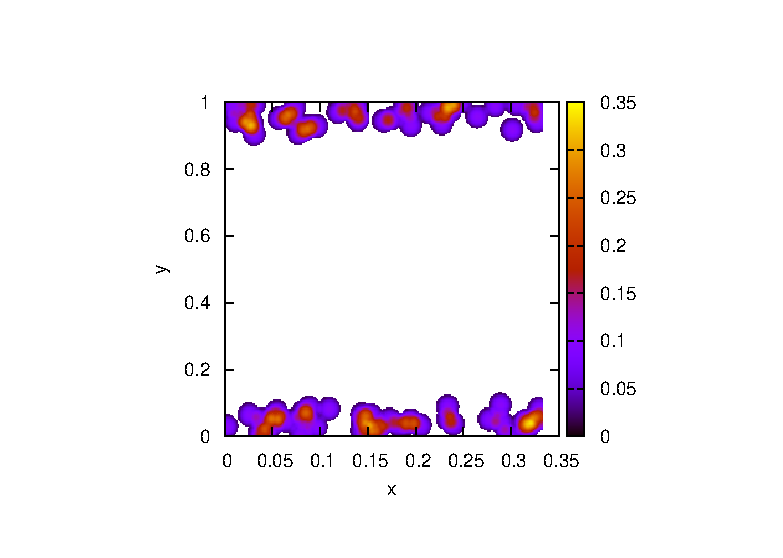
\includegraphics[scale=0.55]{typical_t0.eps} &
      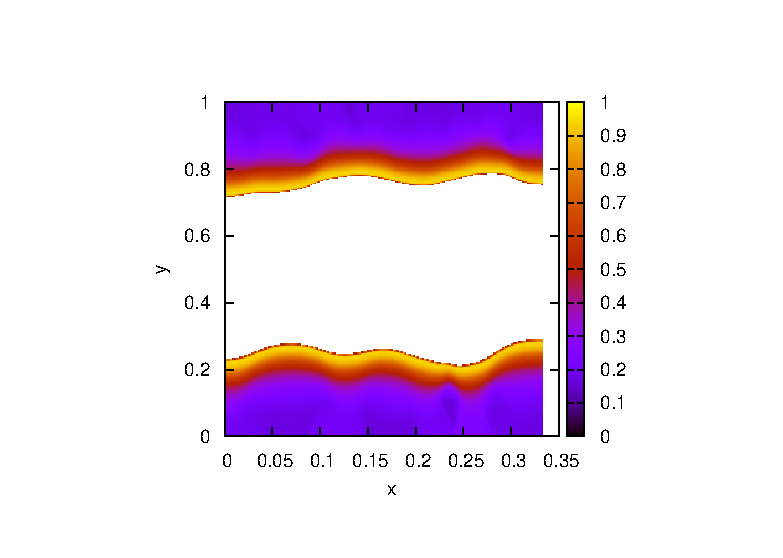
\includegraphics[scale=0.55]{typical_t2.eps} \\
      $t = 0$ & $t = 2$ \\
      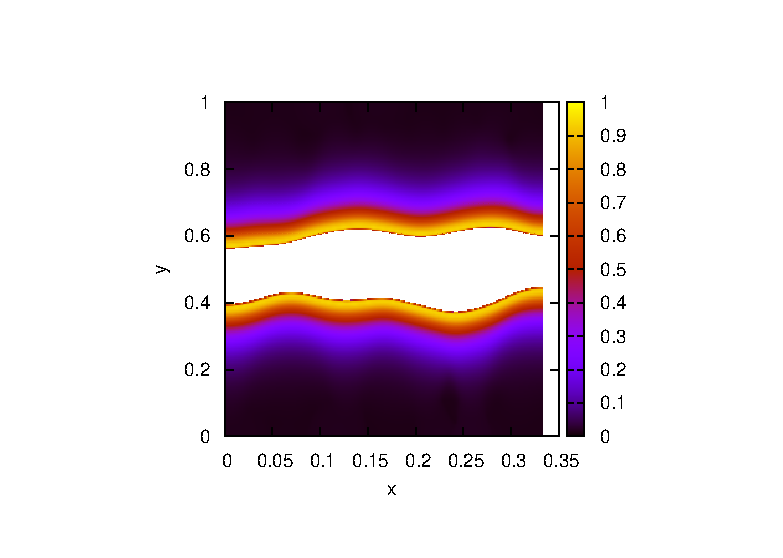
\includegraphics[scale=0.55]{typical_t3_67.eps} &
      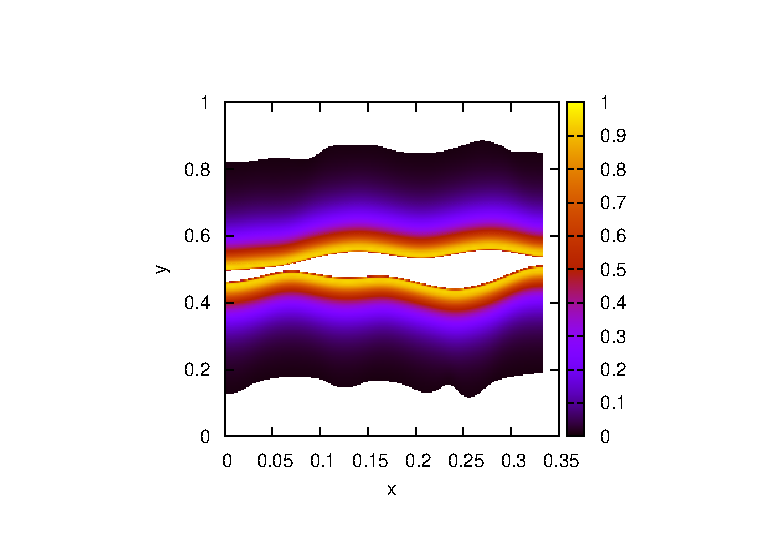
\includegraphics[scale=0.55]{typical_t5_33.eps} \\
      $t = 3.67$ & $t = 5.33$ \\
      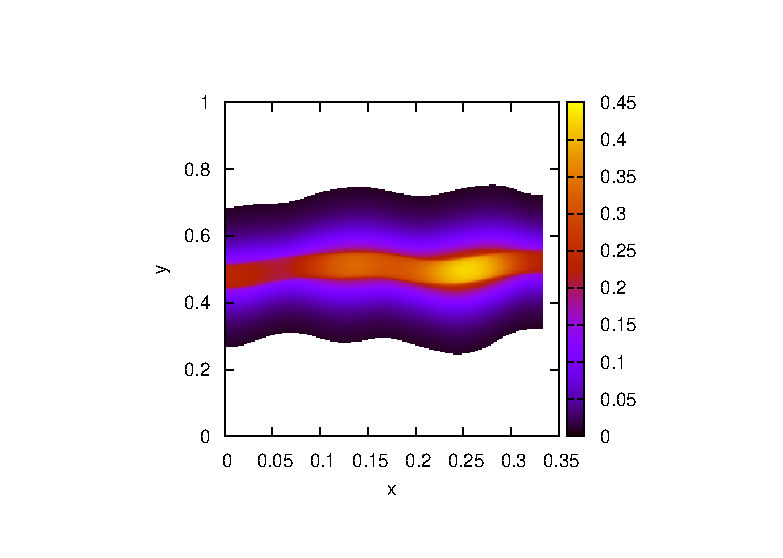
\includegraphics[scale=0.55]{typical_t7.eps} &
      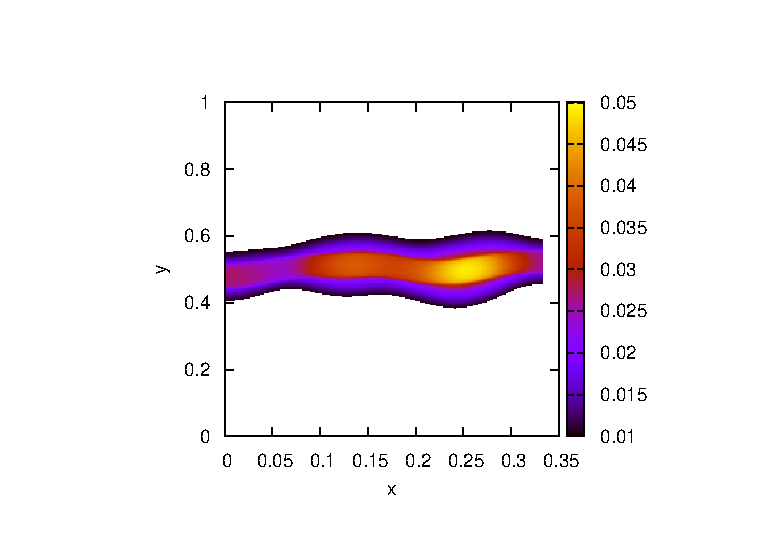
\includegraphics[scale=0.55]{typical_t9.eps} \\
      $t = 7$ & $t = 9$
   \end{tabular}
  \caption{A graph showing the $M$ solution of a typical simulation at different time steps.
    The initial condition is $80$ random spherical inoculation points evenly divided between each of the $y=0$ and $y=1$ sides.
    A $513 \times 513$ grid was used.  }
  \label{fig:typical_sim}
\end{figure}

Figure \ref{fig:typical_sim} shows the time evolution of $M$ for the simulation.
Here, the random inoculations on both sides of the region propagate towards each other and eventually combine at the center.
By looking at $t=2$, $t=3.67$, and $t = 5.33$ it appears as though the wave front is moving with a constant shape and at a constant speed.
This suggest that there may be the existence of a travelling wave solution which will be explored in the next section.

One important feature to notice is that the time evolution in Figure \ref{fig:typical_sim} matches the conceptual model proposed in \cite{dumitrache2015mathematicalModeling}.
This model can be seen in Figure \ref{fig:alex_schema}.
The different stages of the conceptual model can be observed in our simulation results: 
\begin{itemize}
  \item Stage I: $t = 2$ and $t = 3.67$ show the biomass growing towards the center of the sheet, which is the center white area.
  \item Stage II/III: $t = 5.33$ shows the consumed substrate region as the outer white.
  \item Stage IV: Not shown. Only occurs at the moment when the two bands first collide and the biomass concentration at that point still remains at the actual carrying capacity.
  \item Stage V: $t = 7$ and $t = 9$ show the combined center band, now at a biomass concentration lower then the actual carrying capacity.
\end{itemize}

\begin{figure}[!htp]
  \centering
  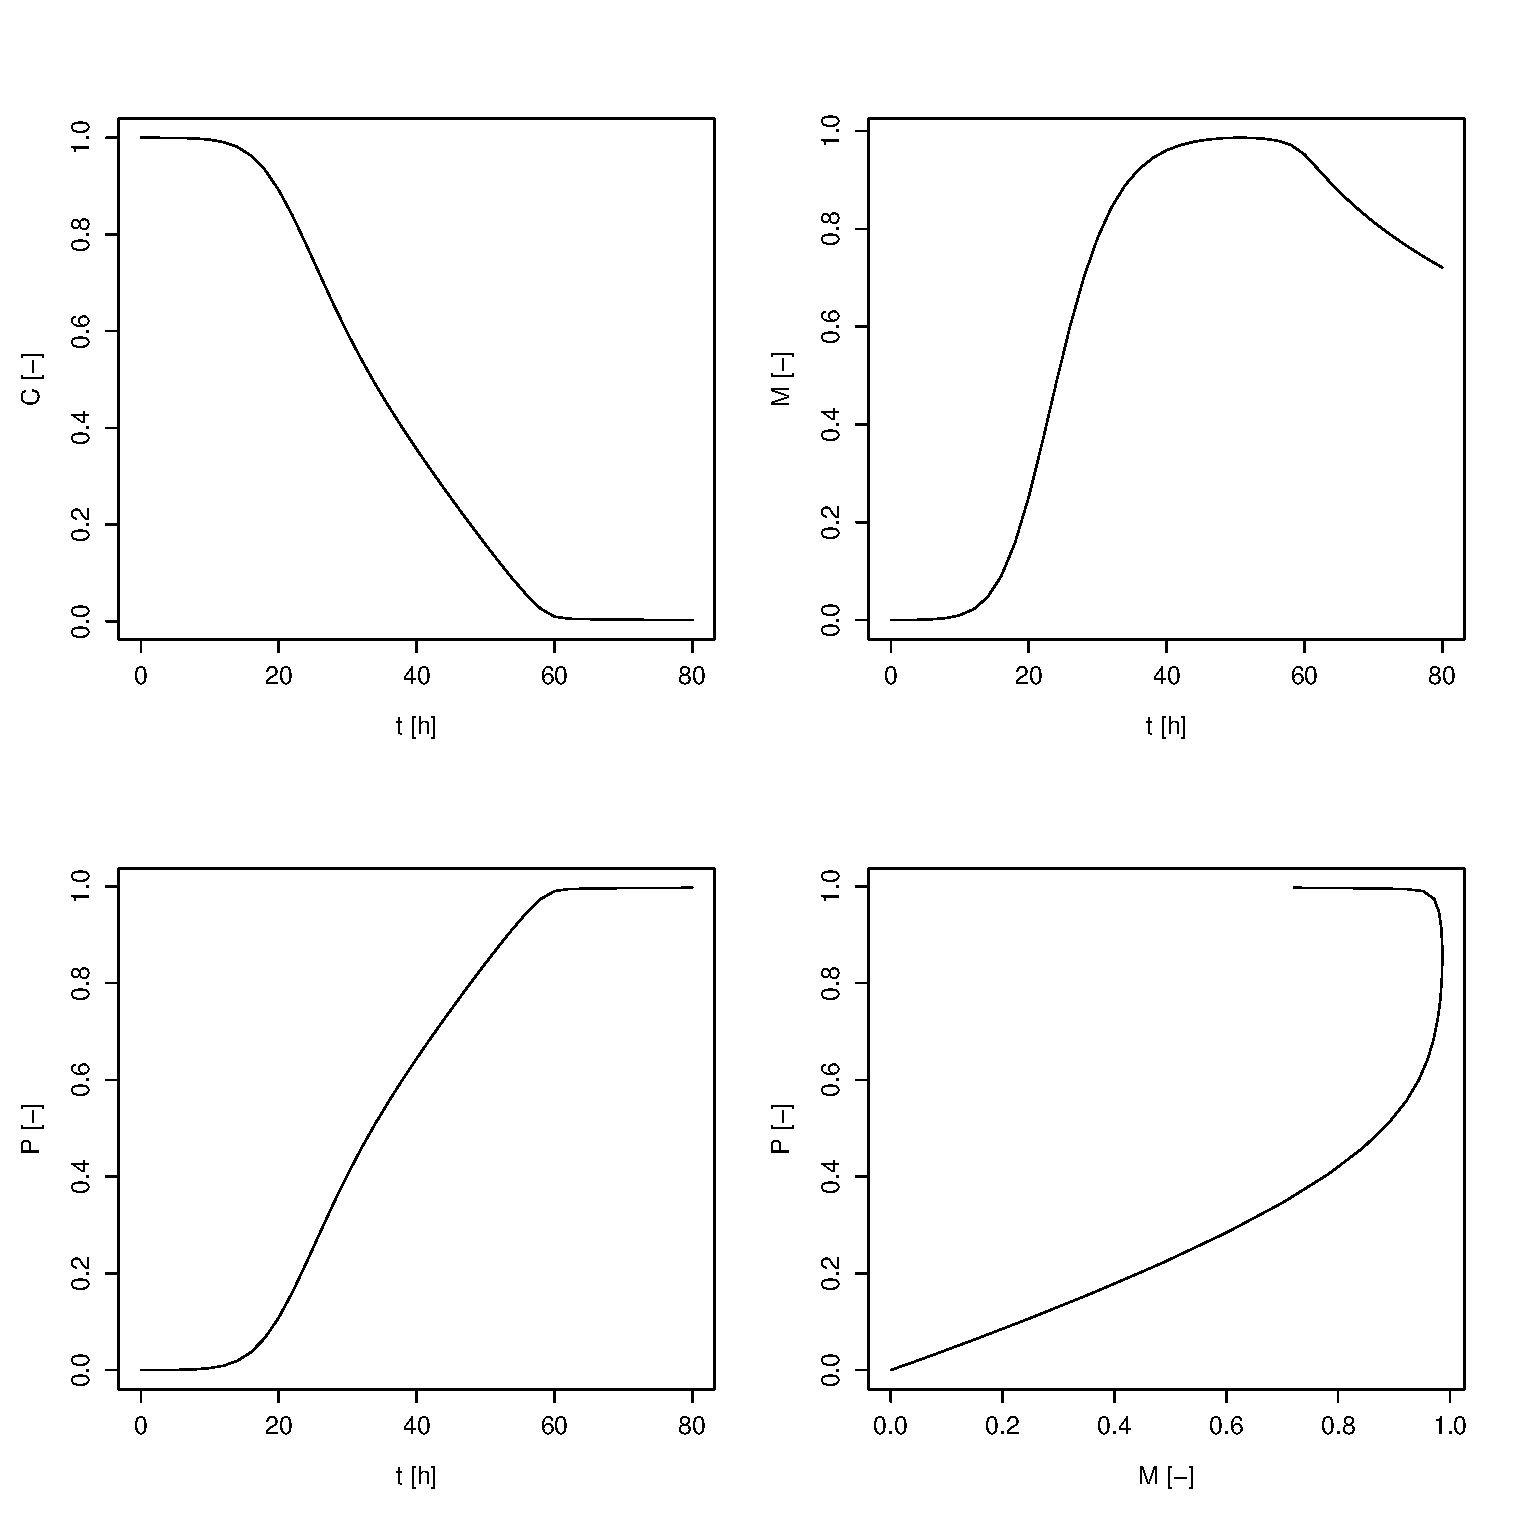
\includegraphics[scale=0.6]{alex_ode_results.eps}
  \caption{A typical model simulation from the simple ODE model.
    Shown are substrate concentration $C$ (top left, normalised), effective sessile biomass $M$ (top right, relative to the ideal carrying capacity $M_{\infty}$), and $CO_2$ product $P$ (bottom left, in moles) as functions of time $t$;.
    Also shown is the product $P$ vs sessile biomass $M$ (bottom right, in moles).
    Figure originally from \cite{dumitrache2015mathematicalModeling}.
  }
  \label{fig:alex_ode_results}
\end{figure}

\subsection{$CO_2$ Production}

Some important quantities to track are the total amount of biomass, $M$, and substrate, $C$. 
%!% HERB: _T_h_e_s_e__v_a_l_u_e_s_ <- Approximations via discretization??
These approximations across the discretization will be called $T_M(t)$ and $T_C(t)$ to represent the total biomass and total substrate, respectively.
The computation for these values can be done by integrating over the region, $\Omega$:
\begin{equation}
  T_M(t) = \int_{\Omega} M dA, \quad T_C(t) = \int_{\Omega} C dA
\end{equation}
These values can be seen in Figure \ref{fig:typical_total} (bd) for $T_M(t)$ and (c) for $T_C(t)$.

\begin{figure}[!htp]
  \centering
  \begin{tabular}{c c}
    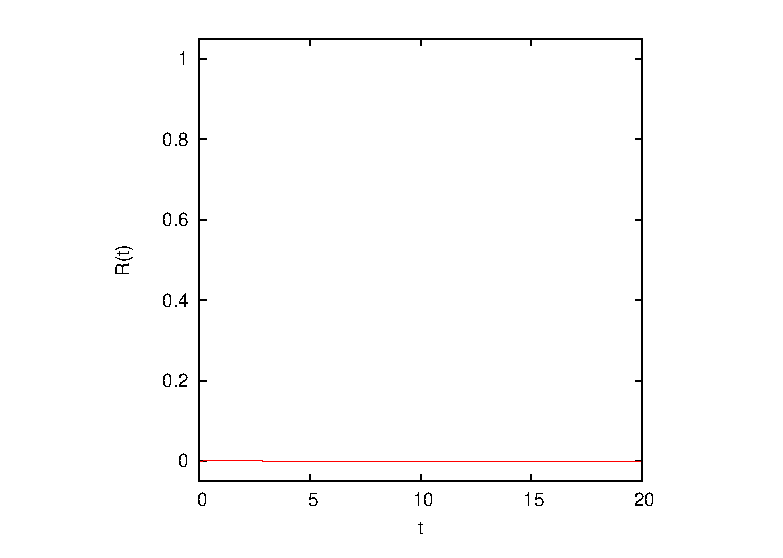
\includegraphics[scale=0.6]{typical_CO2.eps} &
    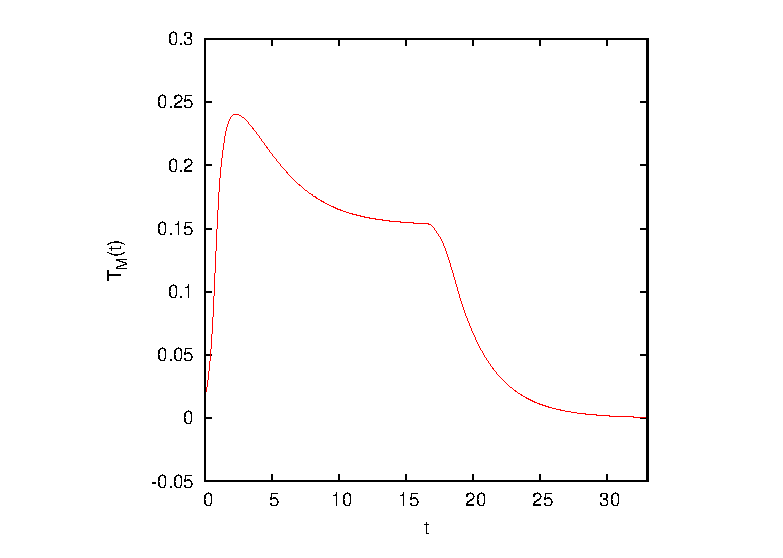
\includegraphics[scale=0.6]{typical_total_M.eps} \\
    (a) & (b) \\
    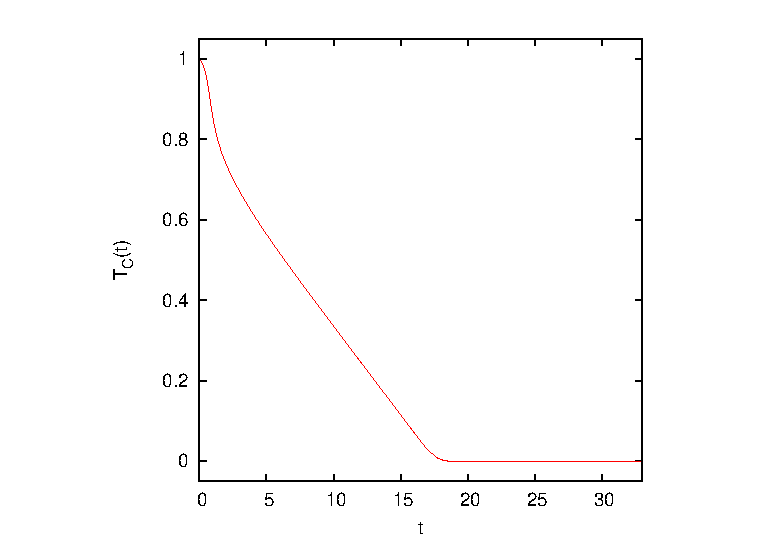
\includegraphics[scale=0.6]{typical_total_C.eps} &
    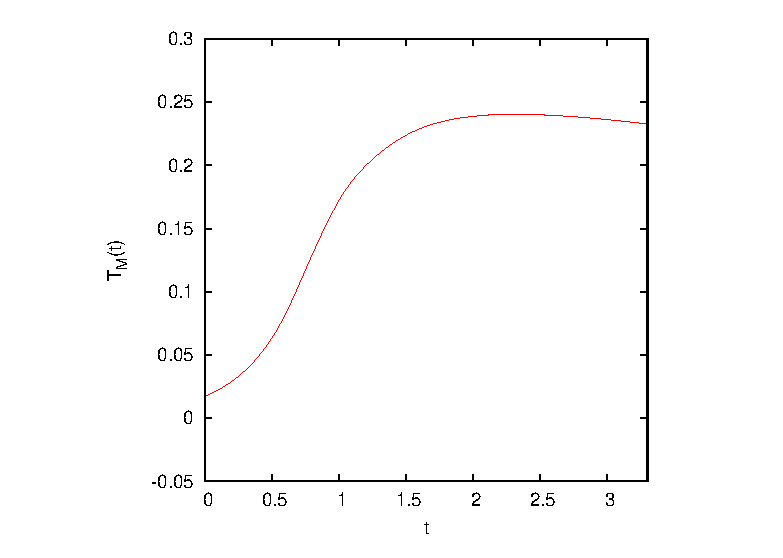
\includegraphics[scale=0.6]{typical_total_M_zoomed.eps} \\
    (c) & (d) \\
    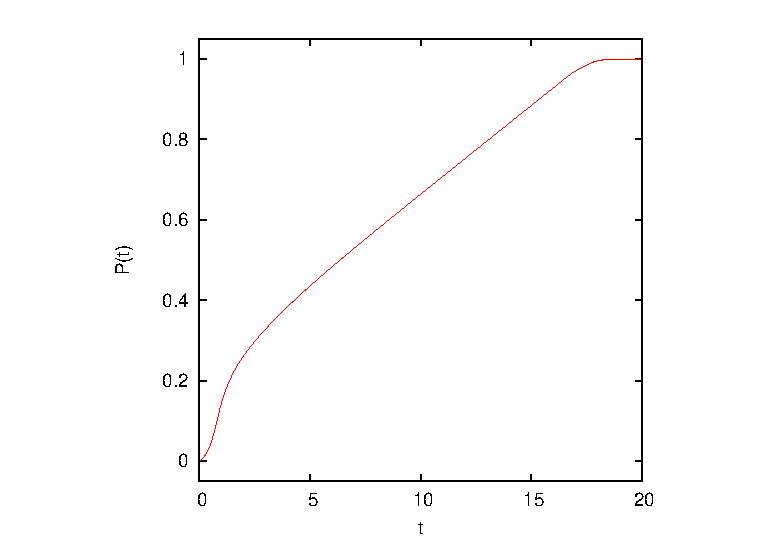
\includegraphics[scale=0.6]{typical_CO2_total.eps} & 
    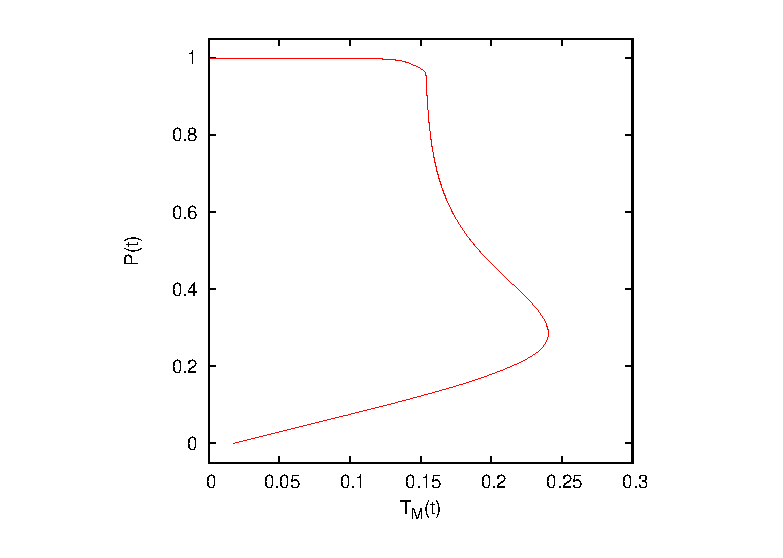
\includegraphics[scale=0.6]{typical_total_PvM.eps} \\
    (e) & (f)
  \end{tabular}
  \caption{Total value of certain qualities from the typical simulation.
    %!% Sometime get this (abcedf) list as an enumerate within the caption... forgot how to do this so look it up later
    Here we have:
    (a) $\mathcal{R}(t)$, the rate of $CO_2$ production,
    (b) total $M$ as a function of time,
    (c) total $C$ as a function of time, 
    (d) total $M$ as a function of time zoomed in from $t = 0$ to $t = 3$,
    (e) $\mathcal{P}(t)$, the total $CO_2$ produced, 
    (f) $\mathcal{P}(t)$ as a function of total $M$.
    All the graphs are from the same simulation with initial condition of $40$ random spherical inoculation points along the $y=0$ side of the region and another $40$ on $y = 1$. 
    A grid of $257 \times 257$ was used for this graph.
    Default parameter set (Appendix A) was used except for $\delta = 10^{-8}$.
  }
  \label{fig:typical_total}
\end{figure}

Since \textit{C. thermocellum} produces $CO_2$ as the substrate is consumed, we can track the production of $CO_2$.
Following the idea from \cite{dumitrache2015mathematicalModeling}, we can equate the change in production of $CO_2$ as time changes by the following equation:
\begin{equation} \label{equ:rho}
p_t = \rho G(C) M.
\end{equation}

To get the amount of $CO_2$ produced at a specific time we get,
\begin{equation}
  \mathcal{R}(t) = \int_\Omega p_t dA = \int_\Omega \rho G(C) M dA.
\end{equation}
From this we can get the more useful value, the total $CO_2$ produced until this point.
\begin{equation}
  \mathcal{P}(t) = \int^t_0 \mathcal{R}(s) ds.
\end{equation}

The $CO_2$ amount is calculated by letting $\rho = 1$ and using the numerically computed values for $G(C)M$ as a measure.
For the same simulation as Figure \ref{fig:typical_sim}, the $CO_2$ information can be seen in Figure \ref{fig:typical_total} (a e).

The results from Figure \ref{fig:typical_total} (c d e f) seems to match the results from the ordinary differential equation model proposed in \cite{dumitrache2015mathematicalModeling}.
Their results can be seen in Figure \ref{fig:alex_ode_results}.
It is important to note that in our system $T_M = 1 $ means that $\Omega$ is completely filled with biomass.
However, in \cite{dumitrache2015mathematicalModeling} they scaled the biomass to the ideal carrying capacity of biomass, i.e. they have $T_M = 1$ when all the biomass is in stage II or III.
The overall result from this experiment is that the spatial two dimension model confirms the conceptual model from \cite{dumitrache2015mathematicalModeling} based on which the reactor-scale model was formulated.
The reactor-scale model consolidated the spatial effects into the carrying capacity of the growth and yet still managed to agree with the results of the actual spatial model.

